\documentclass[slidestop,compress,mathserif,blue,12pt,adobefonts]{beamer}
\usepackage{ctex}
\usepackage{verbatim}
\usepackage{threeparttable}
\usepackage{listings}
\usetheme{Antibes} 
\usecolortheme{lily}
\mode<presentation>


\setCJKfamilyfont{song}{Adobe Song Std}
\setCJKfamilyfont{zhongsong}{Adobe Song Std}
\setCJKfamilyfont{kai}{Adobe Kaiti Std}
\setCJKfamilyfont{hei}{Adobe Heiti Std}
\setCJKfamilyfont{fs}{Adobe Fangsong Std}
\setCJKfamilyfont{li}{Adobe Kaiti Std}
\setCJKfamilyfont{yy}{Adobe Fangsong Std}
\newcommand{\song}{\CJKfamily{song}}
\newcommand{\zs}{\CJKfamily{zhongsong}}
\newcommand{\kai}{\CJKfamily{kai}}
\newcommand{\hei}{\CJKfamily{hei}}
\newcommand{\fs}{\CJKfamily{fs}}
\newcommand{\li}{\CJKfamily{li}}
\newcommand{\yy}{\CJKfamily{yy}}
%\setmainfont{Arial}
% \renewcommand{\familydefault}{\sfdefault}
\setmainfont{Times New Roman} %英文字体使用Times New Roman


\lstset{
	language=bash,
	numbers=left,
	numberstyle=,
	numbersep=10pt,
	basicstyle=\scriptsize,
	%frame=shadowbox, % single,
	tabsize=4,
	breaklines=true,
	emptylines=2,
	keywordstyle=\color{blue!70},
	commentstyle=\color{red!50!green!50!blue!50},
	rulesepcolor=\color{red!20!green!20!blue!20},
	stringstyle=\ttfamily,
	%backgroundcolor=\color{yellow!5!red!5}
}

\def\code#1{\lstinline[basicstyle=\ttfamily,keywordstyle=\ttfamily]{#1}}


  \title{基于模拟退火算法的\\虚拟机部署问题}
  \author{钱~行 \\ 指导教师: 钱柱中}
  \institute{南京大学~~计算机科学与技术系}

\usepackage{fontspec,xunicode,xltxtra}	% must be placed last

\begin{document}


\begin{frame}
  \titlepage
\end{frame}

\begin{frame}
  \frametitle{提纲}
  \tableofcontents
\end{frame}

\section{研究背景}
\begin{frame}
  \frametitle{云计算和虚拟化技术}
  \begin{enumerate}
  \item<1-> 云计算是热点问题
  \item<2-> Amazon等公司的成功
  \item<3-> 虚拟化技术(虚拟机部署问题)是核心
  \end{enumerate}  
\end{frame}


\begin{frame}
  \frametitle{虚拟机部署问题}
  \begin{itemize}
  \item <1->装箱问题(Bin Packing Problem)
  \item <1- |alert@2>NP-Complete
  \end{itemize}
\end{frame}

\section{基于内存共享的虚拟机部署技术}
\begin{frame}
  \frametitle{资源的不同特点}
  \begin{enumerate}
  \item <1- |alert@1> 内存资源的可共享性
  \item 会发生冲突
  \end{enumerate}
\end{frame}

\begin{frame}
  \frametitle{问题定义}
  \begin{itemize}
  \item 输入:虚拟机请求序列,$VM_i = \{\ C^{\thinspace req}_i,R^{\thinspace req}_i,\gamma_i\ \}$
  \item 输出:该序列的一个划分
  \item 目标:该划分尽可能``好''
  \end{itemize}
\end{frame}

\begin{frame}
  \frametitle{优化的依据:评价函数}
  \begin{itemize}
  \item <1->减少PM的使用
  \item <2->均衡负载
  \item <3->减少冲突(平均冲突率的定义)
    \begin{itemize}
    \item 通过约束条件确定阈值
    \item 通过评价函数引导算法
    \end{itemize}
  \end{itemize}
\end{frame}

\subsection{算法设计}

\begin{frame}
  \frametitle{算法设计}
    \begin{enumerate}
    \item <1-> 基于模拟退火算法(simulated annealing)
    \item <1-|alert@1> 概率模型:在迭代中以一定概率接受坏解
    \end{enumerate}
\end{frame}

\begin{frame}
  \frametitle{实现}
  \begin{enumerate}
  \item Python
  \item 参数的设置
    \begin{itemize}
    \item 初始温度
    \item 降温速度
    \item 评价函数
      \begin{itemize}
      \item PM的数量
      \item CPU和内存的负载均衡(均方差)
      \item 平均冲突率\\
         $\rhd$冲突只会发生在过载的PM上\\
         $\rhd$因此算法会在PM数量和平均冲突率上寻求平衡
      \end{itemize}
    \end{itemize}
  \item 测试数据的选取
  \end{enumerate}
\end{frame}


\subsection{实验结果与结论}
\begin{frame}
  \frametitle{算法有效}
  \begin{figure}[htbp]
    \centering 
    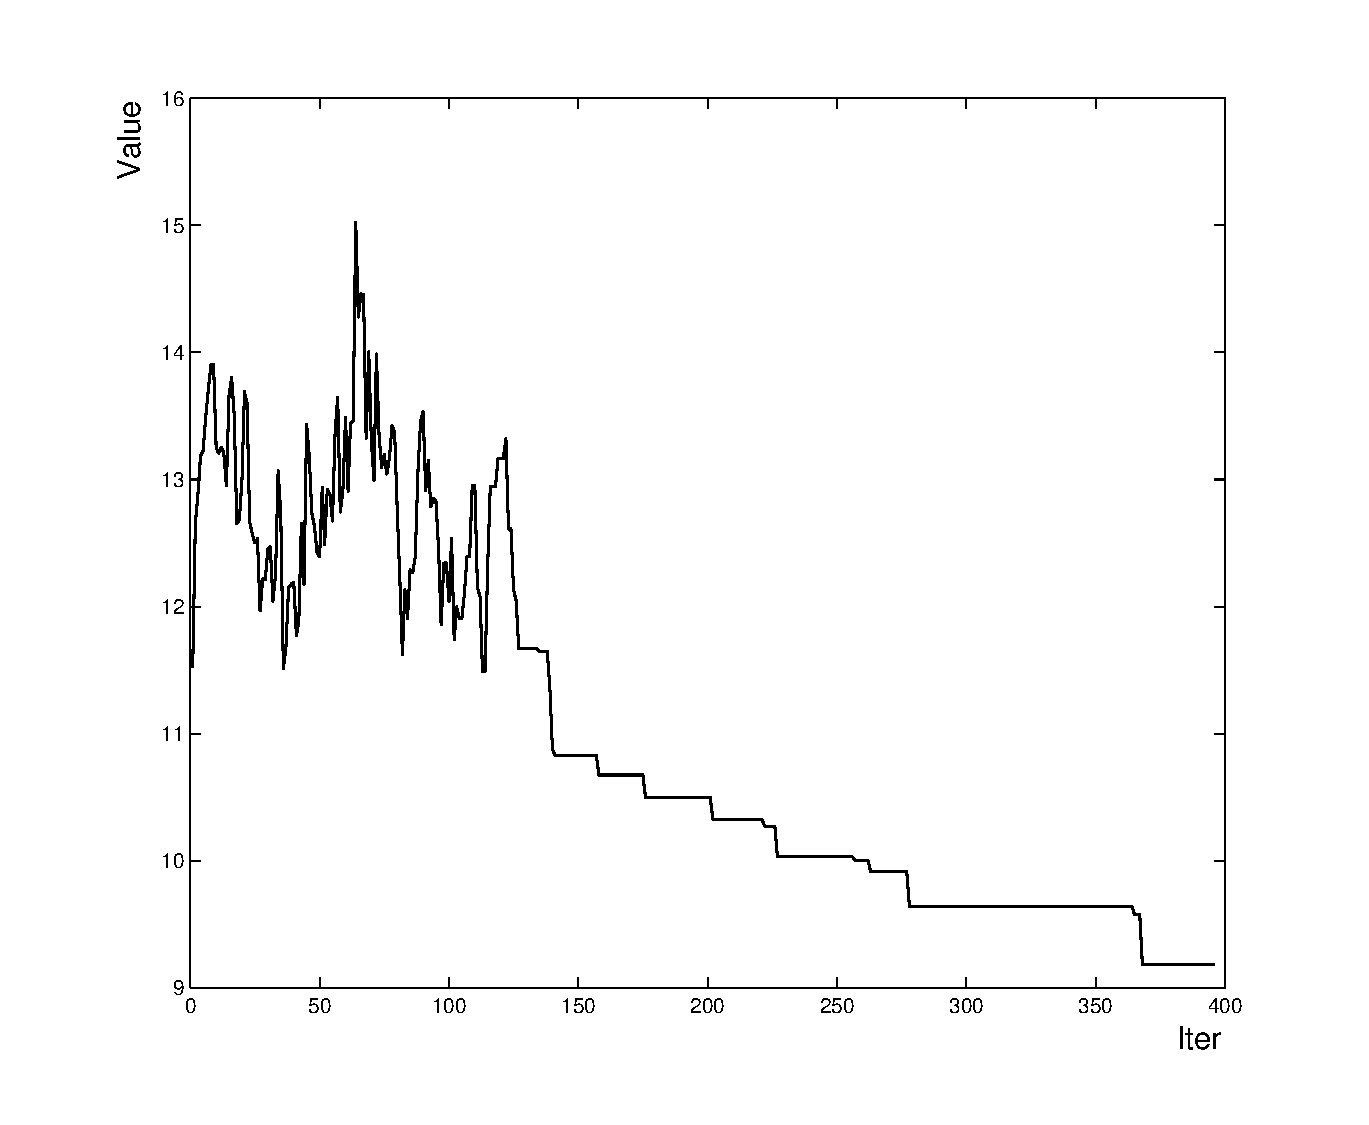
\includegraphics[scale=0.2]{../figures/feasibility.eps}
    \caption{算法收敛}
  \end{figure}
  \begin{itemize}
  \item 算法是稳定的
  \item 收敛+稳定=有效
  \end{itemize}
\end{frame}

\begin{frame}
  \frametitle{结论}
  \begin{enumerate}
  \item <1-> 共享内存有效减少了PM的使用($12\%$)
  \item <2-> 同时能够获得负载均衡的解
  \item <3-> 将平均冲突率控制在可接受范围内($10\%$)
  \end{enumerate}
\end{frame}

\section{总结}
  \begin{frame}
    \frametitle{总结与展望}
    \begin{enumerate}
    \item 引入了内存共享的机制
    \item 控制了伴随的冲突问题
    \item 使用启发式算法
    \item 收到了良好的效果
    \end{enumerate}

    \begin{enumerate}
    \item 对冲突的刻画和避免仍有很大的改善空间
    \item 当冲突发生时如果动态解决
    \end{enumerate}

  \end{frame}

  \begin{frame}
    \vspace{4em}
    \begin{center}
      {\Huge 谢谢!}      
    \end{center}
  \end{frame}

\end{document}

